% This is samplepaper.tex, a sample chapter demonstrating the
% LLNCS macro package for Springer Computer Science proceedings;
% Version 2.20 of 2017/10/04
%

\documentclass[runningheads]{llncs}
%
\usepackage{graphicx}
\usepackage{algorithm}
\usepackage[spanish]{babel}
\usepackage[noend]{algpseudocode}


\begin{document}
%
\title{GATO$\times$GATO}
%
%\titlerunning{Abbreviated paper title}
% If the paper title is too long for the running head, you can set
% an abbreviated paper title here
%
\author{Moreno Ramírez, Eliú\inst{1}}
%
\authorrunning{Eliú Moreno}
% First names are abbreviated in the running head.
% If there are more than two authors, 'et al.' is used.
%
\institute{Instituto Nacional de Astrofísica Óptica y Electrónica, Puebla; México
\email{eliu.moreno@inaoep.mx}\\}
%
\maketitle              % typeset the header of the contribution
%
\begin{abstract}
One of the first approaches to artificial intelligence was through the search mainly in games where for the first time the human faced a computer, one of the most recognized search algorithms is the minimax as well as its alpha-beta variant, so using these algorithms, it is proposed to implement a game, which is a more complex version of the classic cat game, which was called Gato$\times$Gato.

\keywords{Minimax  \and Alpha-Beta \and Búsqueda \and Inteligencia artificial \and Gato$\times$Gato}
\end{abstract}
%
%
%
\section{Introducción}
La habilidad de jugar es considerada como una distincion de inteligencia, debido a la facilidad de crear situaciones complicadas con reglas sencillas, así como la complejidad para ganar se requieren de estrategias ya que se tiene de un oponente impredecible donde es necesario especificar un movimiento para cada respuesta posible del oponente, con este hecho, existe la teoría de juegos, la cual se centra en el estudio estratégico de toma de desiciones. Una manera de tomar dichas desiciones es a través de las técnicas de búqueda los cuales constituyen una representación del conocimiento, que a través de diversos algoritmos nos permite resolver ciertos problemas desde el punto de vista de la inteligencia o para el proposito de este documento la inteligencia artificial. 


\subsection{Motivaciones}
Los juegos de mesa, desde su principio han servido de entrenamiento para la humanidad, debido a que conforme se an ido a evolucionado los juegos en complejidad estos se vuelven un reto para la mente. Con forme algoritmos de busqueda se han ido mejorando, junto con el aprendizaje auomático y con la ayuda de que las computadoras superan los límites del cálculo se han aprovechado los recursos y avances para intentar resolver muchos juegos tales como: go, ajedrez, poker, damas inglésisas, gato, entre otros. 
Unos de los grandes logros de la inteligencia artificial (IA) son:
\begin{itemize}
    \item Damas inglesas: Chinook derrotó al campeón mundial MarionTinsley en 1994. Usó una base de datos de fines de juegos precalculados definiendo jugadas perfectas involucrando 8 o menos piezas en el tablero, un total de 444 mil millones de posiciones
    \item Chess: Deep Blue derrotó al campeón mundial Garry Kasparov en un encuentro de seis juegos en 1997. Deep Blue busca 200 millones de posiciones por segundo y extiende su búsqueda 40 jugadas.
    \item Go: en el años 2016 en Corea Lee Seidel, ex-campeón mundial de Go, fue derrotado 4-1 por el software de Google DeepMind.
\end{itemize}

Inclusive actualmente las computadoras ahora da una nueva manera en el análisis así como conceptos estratégicos para los actuales campeones del mundo en diferentes juegos. Con dichos resultados motivó la creación de un algoritmo que de solución (es decir que sea capaz de poder derrotar a un contricante humano) a una variación del juego gato o 3 en raya, su manera de jugar es la siguiente:
\subsubsection{Reglas}
\begin{itemize}
    \item El tablero del juego, consta de 9 tableros clásicos gato, localizados en un tablero de 3x3.
    \item Cada tablero pequeño de gato de $3 \times 3$ lo denominaremos tablero local, y el tablero más grande de $3 \times 3$ lo denominaremos tablero global.
    \item El juego comienza con $X$ jugando donde quieran en cualquiera de los 81 espacios vacíos. Este movimiento manda a su oponente a su ubicación relativa. Por ejemplo, si $X$ jugó en el cuadro superior derecho de su tablero local, entonces $O$ debe jugar a continuación en el tablero local en la parte superior derecha del tablero global. Entonces, $O$ puede jugar en cualquiera de los nueve lugares disponibles en ese tablero local, y cada movimiento envía a $X$ a un tablero local diferente.
    
    \item Si se juega un movimiento para ganar un tablero local según las reglas del gato tradicional, entonces todo el tablero local se marca como una victoria para el jugador en el tablero global. Una vez que un jugador gana un tablero local o se llena por completo, no se pueden jugar más movimientos en ese tablero. Si un jugador es enviado a dicho tablero, entonces ese jugador puede jugar en cualquier otro tablero. El juego termina cuando un jugador gana el tablero global o no quedan movimientos legales, en cuyo caso el juego es un empate.

\end{itemize}
\begin{figure}[h]
\centering
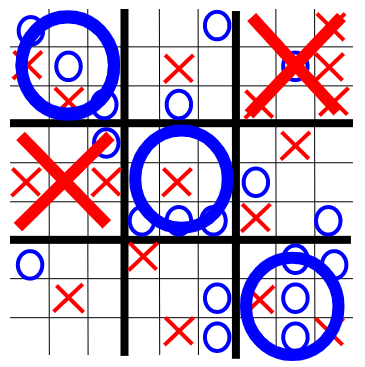
\includegraphics[width=0.35\textwidth]{images/image.png}
\caption{Ejemplo del tablero en una partida ganada por $O$}
\end{figure}
\subsection{Investigación relacionada}
Fernández~\cite{ref_article0} desarrolla un agente de aprendizaje TD para el juego de mesa tres en raya y conecta 4. El agente TD después de jugar un número elevado de juegos contra un oponente (fase de entrenamiento), estas utilidades representan una estimación de la probabilidad de ganar de cada estado. El agente TD busca ir de un estado dado al estado con la mayor utilidad estimada de todos los estados alcanzables en cada juego. Además hacen mención de que un agente de TD al que se le haya enseñado a usar este enfoque puede considerarse un jugador perfecto de tres en raya, ya que nunca ha perdido un juego contra oponentes aleatorios y expertos.

Poliansky~\cite{ref_article1} presenta el uso de la programación genética para evolucionar programas conductuales desde cero, realizando un análisis en profundidad, utilizando como caso de estudio el juego del tres en raya. Menciona que a pesar de que el juego 3 en raya es un problema senciilo no se había abordado antes la evolución para tal dominio. 


\section{Metodología}
Como vemos en el estado del arte el uso de modelos que se entrenan, para resolver estos juegos es una manera que computacionalmente es factible, sin embargo para la implementación de un modelos del juego Gato$\times$Gato que sea capaz de enfrentarse con personas usaremos un algoritmo de busqueda junto con el uso de alguna heurítica. Para la implementación de éste, usaremos una variante del algoritmo minimax Alpha-Beta. 
\subsubsection{Algoritmo minimax}
En teoría de juegos Minimax es un método de decisión para minimizar la pérdida máxima esperada en juegos con adversario y con información perfecta. El funcionamiento de Minimax puede resumirse a como elegir el mejor movimiento para ti mismo; suponiendo que tu contrincante tirará de manera óptima, es decir nos enfrentamos contra un oponente perfecto. Lo que se maximiza es una función, llamada función de evaluación, la cual debe reflejar información de la partida, como posiciones de partida, fichas, movimientos favorecibles a un jugador, entre otras, cabe mencionar que dependiendo de cómo definamos dicha función, el algoritmo de comportará mejor o peor a la hora de maximizar, minimizar. Por lo tanto este algoritmo crea un árbol donde las hojas se etiquetan con gana, pierde, empata, desde el punto de vista de max, con ayuda de una heurística podemos etiquetar cada nodo del árbol, y el jugador max elegirá su movimiento, buscando en árbol un nodo terminal que lo lleve a la posición más favorable que puede esperar desde un estado $J(actual)$ del juego,  suponiendo que el jugador mín juega de manera ideal.
En la práctica el método Minimax es impracticable excepto en supuestos sencillos. Realizar la búsqueda completa requerirían cantidades excesivas de tiempo y memoria. El pseudocódigo de este algoritmo es el que encontramos en $Algorithm$ \ref{alg:1}.

\subsubsection{Mejora de minimax: Poda alfa-beta}
La poda alfa beta es una técnica de búsqueda que reduce el número de nodos evaluados en un árbol de juego por el algoritmo Minimax. Se trata de una técnica muy utilizada en programas de juegos entre adversarios como el ajedrez, el tres en raya o el Go.
El problema de la búsqueda Minimax es que el número de estados a explorar es exponencial al número de movimientos. Partiendo de este hecho, la técnica de poda alfa-beta trata de eliminar partes grandes del árbol, aplicándolo a un árbol Minimax estándar, de forma que se devuelva el mismo movimiento que devolvería este, gracias a que la poda de dichas ramas no influye en la decisión final.
La búsqueda minimax es primero en profundidad, por ello en cualquier momento sólo se deben considerar los nodos a lo largo de un camino en el árbol.
La poda alfa-beta toma dicho nombre de la utilización de dos parámetros que describen los límites sobre los valores hacia atrás que aparecen a lo largo de cada camino. Dichos parametros son primero $\alpha$ el cual es el valor de la mejor opción hasta el momento a lo largo del camino para $\max$, esto implicará por lo tanto la elección del valor más alto y$\beta$ es el valor de la mejor opción hasta el momento a lo largo del camino para $\min$, esto implicará por lo tanto la elección del valor más bajo.
Esta búsqueda alfa-beta va actualizando el valor de los parámetros según se recorre el árbol. El método realizará la poda de las ramas restantes cuando el valor actual que se está examinando sea peor que el valor actual de $\alpha$ o $\beta$ para $\max$ o $\min$, respectivamente.El pseudocódigo de este algoritmo es el que encontramos en $Algorithm$ \ref{alg:2}.
\begin{algorithm}[H]
\caption{Algoritmo minimax}\label{alg:1}
\begin{algorithmic}
\If{si $J$ es terminal}
    \State $V(J)\gets evaluacion(J)$
\ElsIf{genera los sucesores de $J:J_1,J_2,...,J_n$}
    \State Evaluar $V(J_1),V(J_2),...,V(J_n)$ de izquierda a derecha
    \If{$J$ es nodo $\max$}
        \State $V(J) \gets \max[V(J_1),V(J_2),...,V(J_n)]$
    \EndIf
    \If{$J$ es nodo $\min$}
        \State $V(J) \gets \min[V(J_1),V(J_2),...,V(J_n)]$
\EndIf
\end{algorithmic}
\end{algorithm}


\begin{algorithm}[H]
\caption{Algoritmo minimax con mejora alpha-beta}\label{alg:2}
\begin{algorithmic}
\State $\alpha \gets -\infty$
\State $\beta \gets \infty$
\If{$j$ Nodo terminal} 
    \State $V(J) \gets evaluacion(J)$
\ElsIf{sean   $J_1, J_2, . . . , J_n$ los sucesores de J}
\State $k \gets 1$
    \If{$j$  es $\max$}
        \State $\alpha \gets  \max [\alpha, V(J;\alpha,\beta)]$
        \If{$\alpha \geq \beta$}
            \State \textbf{return} $ \beta$
        \Else
            \State \textbf{Continua}
        \EndIf
        \If{k=n}
            \State \textbf{return} $\alpha$
        \Else
            \State $k \gets k+1$
            \State \textbf{Continua}
        \EndIf
    \EndIf
    \If{$j$ es $\min$}
        \State $\beta \gets \min[\beta,V(J;\alpha,\beta)]$
        \If{$\beta \leq \alpha$}
            \State \textbf{return} $\alpha$
        \Else
            \State \textbf{Continua}
        \EndIf
        \If{$k=n$}
            \State \textbf{return} $\beta$
        \Else
            \State $k \gets k+1$
            \State \textbf{Continua}
        \EndIf
    \EndIf
\EndIf 
\end{algorithmic}
\end{algorithm}
\subsubsection{Implementación}
Para la implementación del programa como ya hemos dicho se realizará usando el algoritmo mejorado de minimax el cual es alpha beta, éste se realizó en el lenguaje \textit{python}, dicha consiste en las siguientes partes: 
\begin{itemize}
\item Interfaz donde se muestra el dibujo y la interacción de la persona con el tablero, esto se realiza con la librería \textit{pygame}.
\item El árbol de búsqueda, donde se guardan los estados que se pueden desombocar desde uno inicial, el cual debe tener la información de un peso(para el presente trabajo de denominará como score), la posición de cada estado y los turnos de max y min. Esta parte para hacer sensilla la implementación se realizarán listas, ya que es muy sencillo acceder a ella con índices y guardar cualquier tipo de información.
\item Por último la parte fundamenta para el algoritmo alpha-beta es la función de evaluación, la cual debe involucrar toda la información actual de un estado en el juego. Por lo que para el juego Gato$\times$Gato necesitamos de la siguiente información:
\begin{itemize}
    \item Posición del jugador $\max$
    \item Tableros locales ganados por los jugadores $\max$ y $\min$
    \item Tener en cuenta las combinaciones para ganar (por ejemplo las filas, columnas, y las 2 diagonales) tanto para ganar un tablero local, como para el tablero global
\end{itemize}
Por lo que la función propuesta es dar un score, dependiendo la jugada posible, por ejemplo dar un score alto por cada tablero local ganado, un score medio si es posible que en la siguiente jugada se gana un tablero local y además, debido a la manera de jugar es posible que haya marcas más $'X'$ o $'O'$ en un tablero local, es decir generalmente no habrá la misma cantidad de marcas de ambos jugadores en el mismo tablero local, por lo que podemos usar esta información, así que daremos un score bajo dependiendo de cuántas marcas tenga $\max$ en su tablero local actual, siempre y cuando este movimiento no sea un movimiento de los previos mencionados. Por lo que para la implementación de esta función se usó como un score alto, medio, bajo los puntajes 20,3,1 respectivamente. 
\end{itemize}


\section{Discusiones}
El algoritmo alpha-beta se desempeña de buena manera para este juego el cual puede llegar a generar un árbol lo suficientemente grande si se hiciera búsqueda exhaustiva por lo que dicha mejora fue lo más óptimo sin embargo su desempeño no es el mejor en ciertas situaciones, por ejemplo al ejecutar el juego en el momento en que el jugador 'humano' manda a la computadora a un tablero local el cual está o ya ganado o lleno (ver cuadro \ref{tab:1}), la búsqueda de la mejor posición se complica porque en vez de analizar un tablero local, el algoritmo toma en cuenta el resto de los locales, lo cual incrementa el tiempo de elección de mejor movimiento, pero cuando es cualquier otro caso dentro de las reglas, sí es menor el tiempo de ejecución pero aún no es el mejor.
\begin{table}
\begin{center}
\begin{tabular}{| c | c |}
Movimineto & Tiempo (s) \\ \hline
Tablero Local Lleno/Ganado & ~14  \\
Ganar tablero Local & ~5\\
Sencillo &  2 \\ \hline
\end{tabular}
\caption{Tiempo aproximado en que la computadora tarda en decidir movimientos específicos}
\label{tab:1}
\end{center}
\end{table}
\\
\textit{El cuadro \ref{tab:1} se obtuvo tras ejecutar el juego con una persona aproximadamente 50 veces.}

\section{Conclusiones}
Como podemos ver a pesar de ser dicho algoritmo el cual puede desempeñarse bien en la toma de decisiones en juegos, esto nos ayuda siempre como una buena base al momento de implementar un juego nuevo el cual sea un buen reto de jugar humano-máquina, siempre y cuando la función de evaluación sea apropiada para el problema, como vemos en juego implementado Gato$\times$Gato debido la cantidad grande de casillas en el tablero global, al momento de hacer búsqueda puede generar una gran cantidad estados posibles en cada momento de selección y a pesar de que en el presente trabajo se usó una mejora de minimax, para tener una mejor eficiencia, aún así no es lo mejor para este juego, como trabajo futuro se propone encontrar una mejor heurística en la función de evaluación para una mejor elección ya que es importante a discutir la importancia de las casillas es decir, es bien sabido que en los juegos de mesa algunas posiciones ganadas por un jugador son de mayor importancia que otras por ejemplo, en el clásico juego gato, aquel jugador que marcó la casilla de en medio tiene más posibles de ganar que el otro, esto porque si tienes esa marca tienes 4 posibles estados ganadores(que son ganar por una linea horizontal, una vertical y las dos diagonales) de un total de 8 posibles estados que permiten ganar el juego(que son las 3 lineas horizontales, 3 verticales y las 2 diagonales), tomando todas las demás casillas y que al aumentar las posibilidades de ganar tirando en medio disminuye mucho las posibilidades de que el otro jugador gane. Con este precedente es posible que para el Gato$\times$Gato algunas casillas tengan más peso que otras, por lo que sería interesante experimentar con tales hipótesis. Así como el jugar con los pesos de las diferentes tiradas usadas en la implementación, además de usar técnicas de juegos empleadas en el estado del arte como se vio en la investigación relacionada.

% ---- Bibliography ----
%
% BibTeX users should specify bibliography style 'splncs04'.
% References will then be sorted and formatted in the correct style.
%
% \bibliographystyle{splncs04}
% \bibliography{mybibliography}
%
\begin{thebibliography}{8}
\bibitem{ref_article0}
Fernández-Conde, J.; Cuenca-Jiménez, P.; Cañas, J.M. Hybrid Training Strategies: Improving Performance of Temporal Difference Learning in Board Games. Appl. Sci. 2022, 12, 2854. https://doi.org/10.3390/app12062854
\bibitem{ref_article1}
Poliansky, R.; Sipper, M.; Elyasaf, A. From Requirements to Source Code: Evolution of Behavioral Programs. Appl. Sci. 2022, 12, 1587. https://doi.org/10.3390/app12031587

\end{thebibliography}
\end{document}
